\addcontentsline{toc}{part}{Conclusion et Bilan}
\newgeometry{height=10in}.

\chapter*{Conclusion et Bilan}
\setcounter{section}{0}


\section*{Bilan du chef de projet}

\subsection*{Bilan global}
Le projet s'est dans l'emsemble bien déroulé. Le principal problème a été de constamment devoir recommencer les différents diagrammes jusqu'à ce qu'ils soient corrects, et qui a parfois étant un peu décourageant. Il a été difficile de partager efficacement le travail entre les différents membres, et de parraléliser les tâches car la compréhension du projet dans sa globalité était souvent nécessaire pour faire des diagrammes aussi précis et justes que possible.

\subsection*{Outils utilisés}
Comme sur chaque projet, il est important d'utiliser de bons outils pour travailler efficacement et avoir des livrables avec une bonne qualité, et qui évitent de devoir répéter de nombreuses fois les mêmes tâches.\\

Nous n'avons trouvé qu'ils n'existent pas voir peu d'outils qui soient réellement pratiques pour la réalisation de ces projets. En effet, il n'est pas possible de gérer des variables qui soient utilisables entre les diagrammes, puis entre les IHM puis dans le rapport. Si une modification est effectuée en fin de projet, il faut obligatoirement vérifier sa cohérence avec le reste des livrables.\\

Dans le but d'harmoniser l'ensemble du rendu, nous avons choisi d'utiliser \textbf{PlantUML} pour réaliser l'ensemble des diagrammes. La possibilité d'utiliser des variables pour les différents diagrammes nous a permis de détecter et d'éviter les redondances au niveau des services métiers. Le principal problème avec cet outil est qu'il est difficile de s'éloigner de l'UML standard (exemple : impossible de créer plusieurs "\textit{end points}" dans les diagrammes d'activités).\\

Les IHM ont été réalisées à l'aide de \textbf{Balsamiq}, qui est malheureusement un des seuls outils qui permettent d'aller assez rapidement. Mais l'export pdf final est très décevant au niveau qualité. \\

L'ensemble du suivi du projet a été effectué sur \textbf{Redmine}. Nous n'avons pas trop utilisé l'affectatioin des tâches à des personnes car il était nécessaire que plusieurs personnes relisent les différents diagrammes pour s'assurer de leur cohérence avec le reste. Ainsi, seules les tâches principales ont été affectées, et les différents membres de l'équipe devaient indiquer le temps passé sur les différentes tâches sur le \textbf{Redmine}.\\

Le challenge de ce type de projet a été d'assuré une bonne communication globale entre les membres du projet. Nous avons utilisé l'outil collaboratif \textbf{Slack} pour ceci ainsi q'un répertoire \textbf{Git} pour échanger le code \textbf{PlantUML}. Malheuresement, les fichiers d'IHM étaient difficilement \textit{versionables}, et ceci nous empechaient à travailler à plusieurs dessus du fait de la difficulté à fusionner le travail de plusieurs membres.

\subsection*{Bilan sur le temps de travail}
  \begin{figure}[H]
    \begin{tikzpicture}
      \begin{axis}[
        mbarplot,
        ylabel=Temps (Heures),
        axis y line=left,
        axis x line=bottom,
        xmin=0, xmax=5,
        ymin=0, ymax=40,
        xtick={1,2,3,4},
        xticklabels={Conception\\ d’ensemble,Conception\\ fonctionnelle\\ détaillée,Conception\\ applicative\\ détaillée,Architecture\\ technique},%<--Here
        xlabel style={yshift=-1cm},
        x tick label style={
            rotate=62,
            anchor=east,
            font=\footnotesize,
            align=right
        },
        width=\textwidth,
        height=7cm,
      ]

      \addplot plot coordinates {(1, 20) (2, 25) (3, 22.4) (4, 12.4)};
      \addplot plot coordinates {(1, 18) (2, 24) (3, 23.5) (4, 13.2)};

      \legend{Temps estimé, Temps passé}

      \end{axis}
    \end{tikzpicture}
  \end{figure}
  
On trouve ci-dessus un graphique indiquant le temps mis par l'équipe sur chaque tâche (le temps pour la finalisation n'est pas indiqué).
On constate un dépassement du temps estimé pour la réalisation du projet, en particulier du au fait qu'il a fallu recommencer plusieurs fois les diagrammes à cause de certains aspects métiers peu clairs et/ou mal compris (ex : contact prévu/affecté, plusieurs rendez-vous par contact, organisation de la proposition commerciale, etc...)\\

La durée totale a été de \textbf{173} heures (présentation et fin de préparation de la présentation non compris). Ceci correspond à environ \textbf{28} heures par membres de l'équipe du projet, soit environ \textbf{12} heures  de travail par personne en dehors des séances.\\

Les dépassements de temps ont été dûs au fait qu'il fallait une compréhension de la globalité du projet par l'ensemble des membres de l'équipe, car il comprenait de nombreuses petites substilités. De ce fait, les travaux de relectures des travaux et de compréhension des travaux des autres personnes du projet ont entrainé des dépassements de temps sur de nombreuses tâches. Ceci a néanmoins permi d'assurer un travail cohérent dans la globalité, ainsi qu'une meilleur compréhension des problèmes.\\



\begin{figure}[H]
\noindent\makebox[\textwidth]{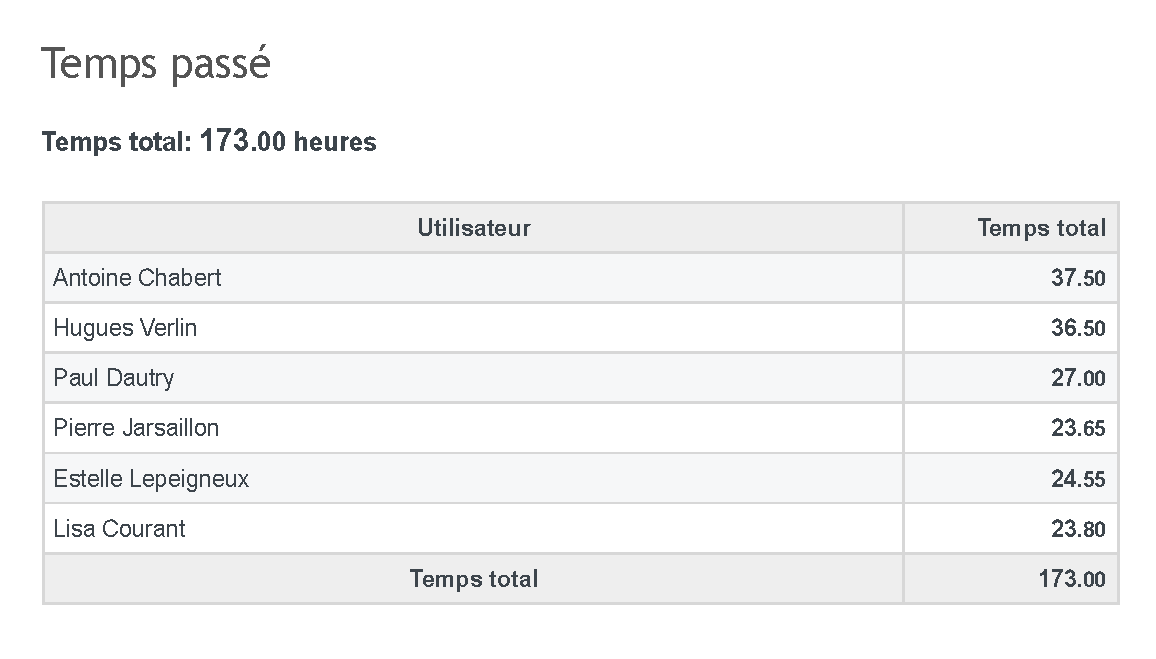
\includegraphics[width=14.5cm]{figures/tempspersonne.pdf}}
\caption{Temps de chaque personne sur le projet}
\end{figure}


On note que la conception fonctionnelle détaillée a occasionée un important dépassement de temps, en raison du fait qu'il a fallu modifier à plusieurs reprises les DSS et les DA en raison d'une mauvaise compréhension du métier au préalable. En effet, il faut un certain laps de temps avant que chaque terme utilisé dans le projet soit assimilé et semble logique (par exemple : contact réalisé/contact prévu, plage agenda, ...).\\

En revanche, la rédaction du rapport a été finalement assez rapide, tout comme la génération du diagramme de collaboration, du fait du travail effectué lors des étapes précédentes.

\section*{Bilan humain et conclusion}
Globalement le projet c’est bien passé. Nous sommes arrivés à termes du projet et nous avons réussi à modéliser l'ensemble des cas d'utilisations.\\

Cependant, nous avons eu quelques points négatifs sur le plan humain. En effet, la gestion du projet via redmine a été un peu lourde pour un petit projet comme celui-ci, et il est un peu long de devoir indiquer à chaque fois le temps mis pour réaliser les différentes tâches du projet. \\

Quelques problèmes de compréhension sont survenus au cours du projet, de même que certaines personnes ont eu du mal à utiliser PlantUML au début. En revanche, tout le monde était content de son fonctionnement à la fin.\\

A la suite de cette partie, le lecteur pourra trouver un tableau récapitulant les différentes tâches du projet. Les durées des tâches principales ont du être recalculées à la main car Redmine ne fait l'addition que sur les temps estimés. 


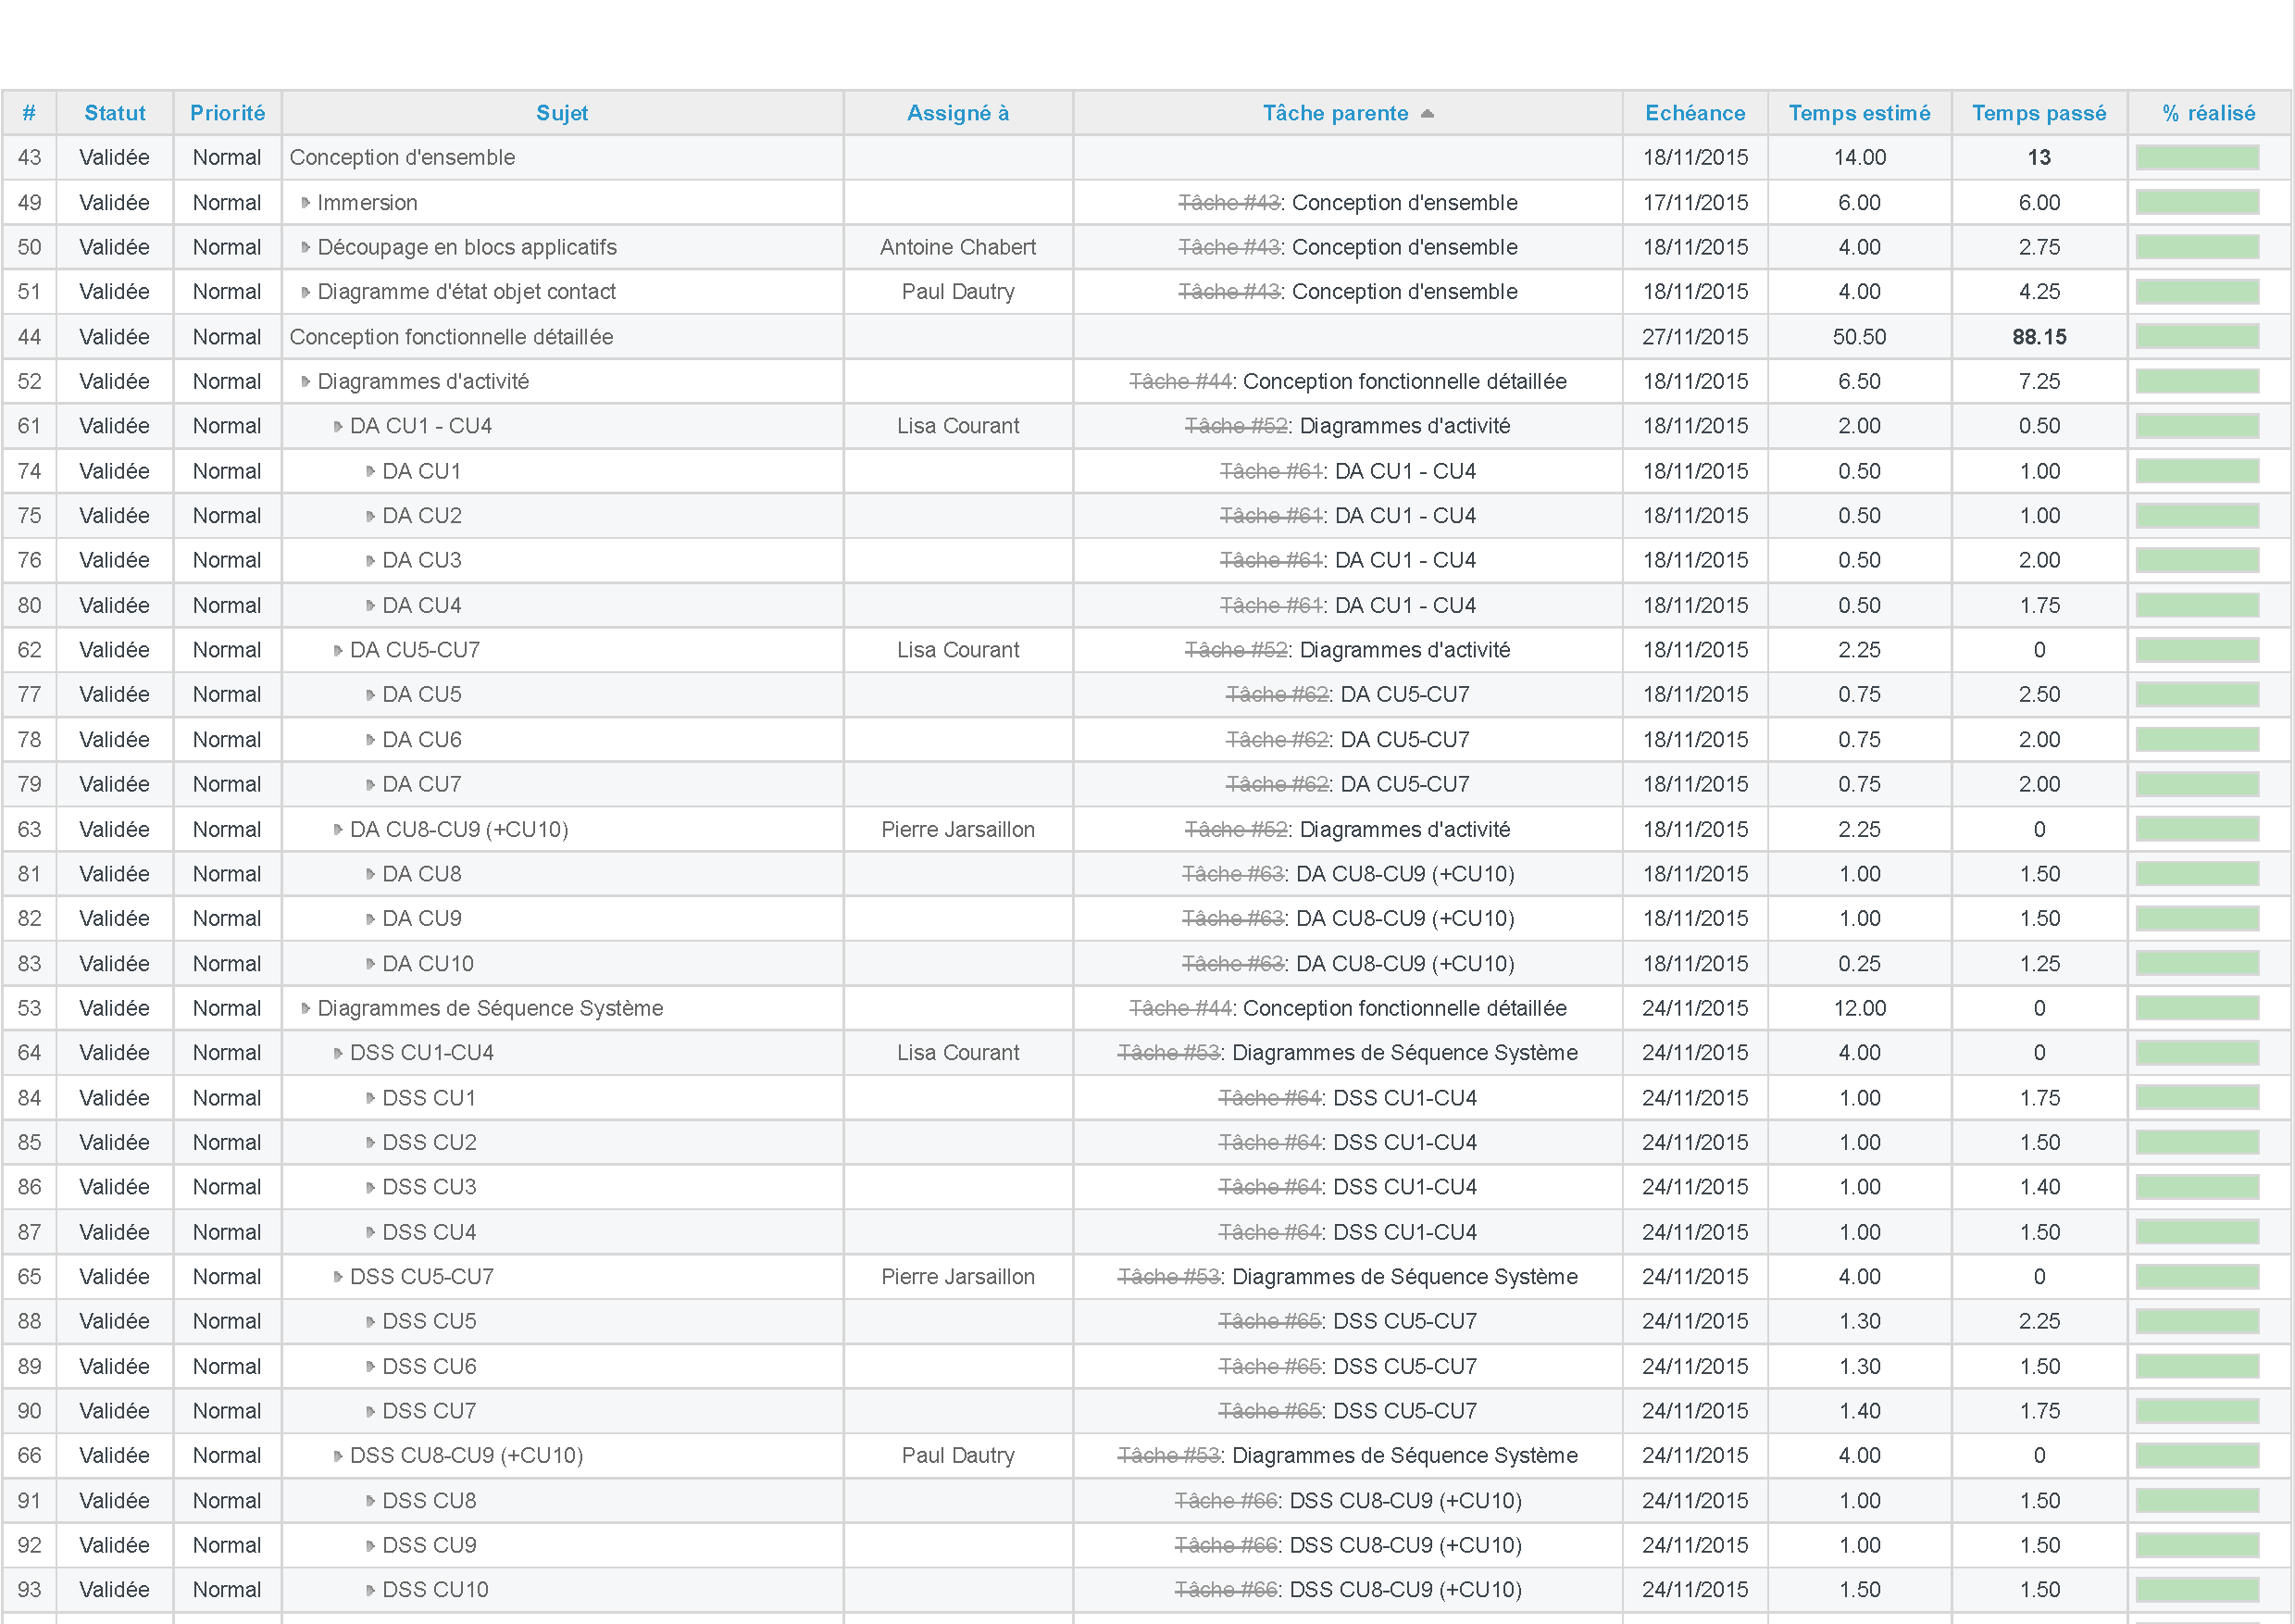
\includepdf[scale=0.8,angle=90,pages=-,pagecommand=\subsection*{Bilan du projet - Export Redmine}]{figures/avancement.pdf}

\begin{figure}[H]
\noindent\makebox[\textwidth]{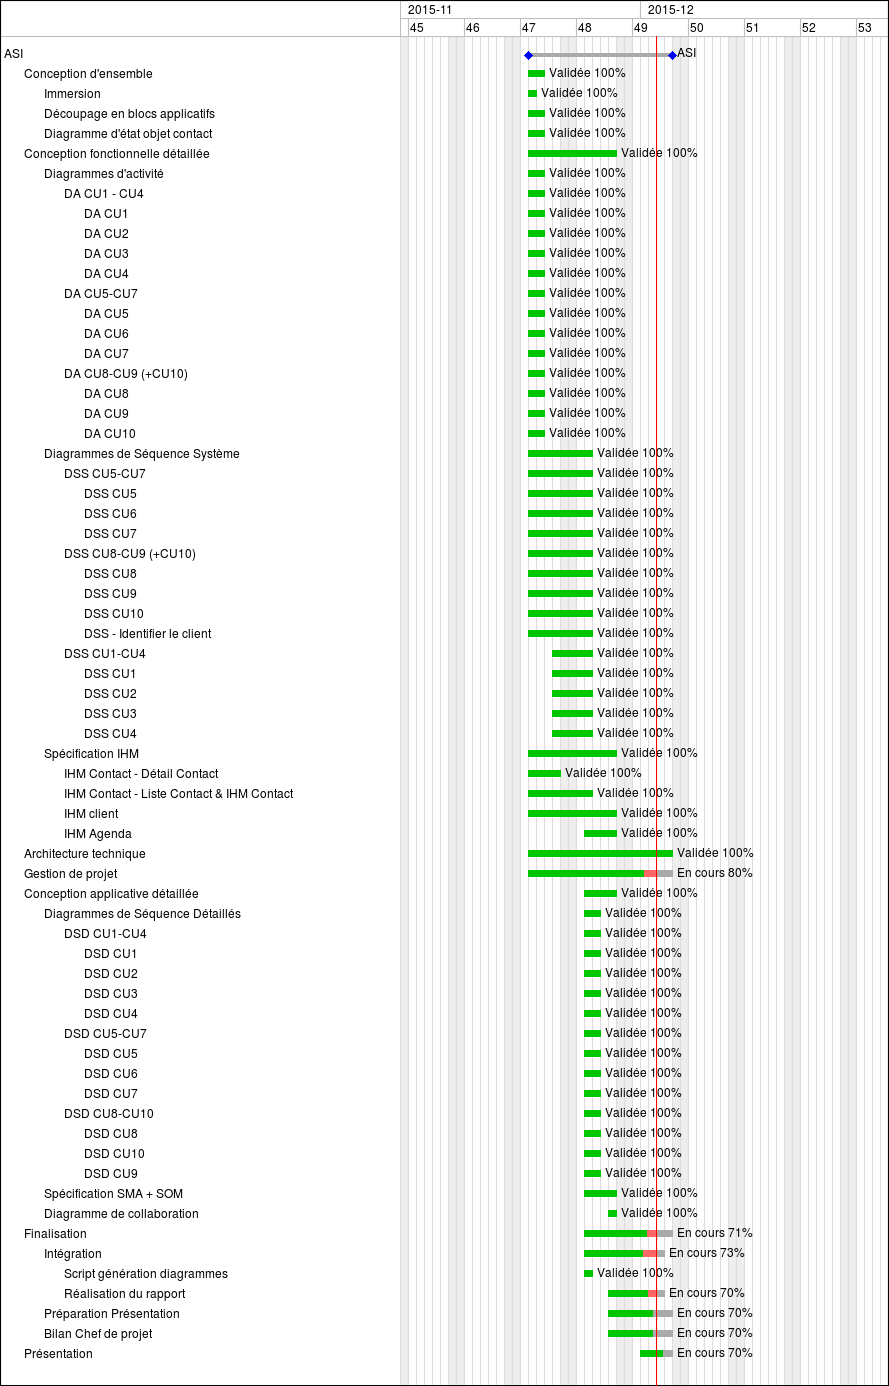
\includegraphics[width=16.5cm]{figures/asi-gantt.png}}
\caption{Gant du projet}
\end{figure}



\restoregeometry